
\section{Self Supervised}
There's a line of research tackling monocular depth estimation from a self-supervised learning approach. Well studied geometric relations implicitly constrain depth maps of subsequent frames in videos or in stereo pairs making it suitable to define self-supervised losses for training, i.e. not dependent on ground truth depth maps.\\

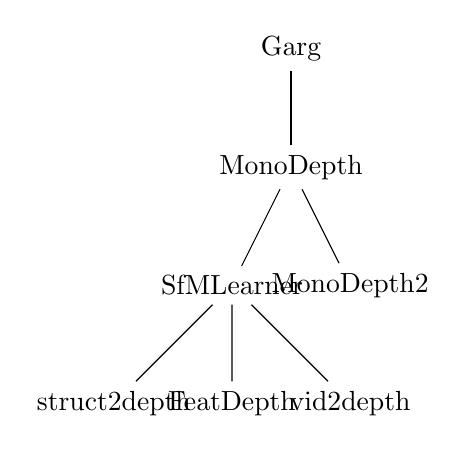
\begin{tikzpicture}
\node{Garg}
	child{node{MonoDepth}
		child{node{SfMLearner}
			child{node{struct2depth}}
			 child{node{FeatDepth}}
			child{node{vid2depth}}
		}
		child{node{MonoDepth2}}
};
\end{tikzpicture}

Garg et al. \cite{Garg} rely on having rectified stereo footage with known baseline and camera parameters. Given a stereo pair $I_{l}, I_{r}$ they feed $I_{l}$ to their depth estimation network which returns an estimate of its depth map $\hat{\rho}_{l}$. After converting $\hat{\rho}_{l}$ to a disparity map $\hat{d}_{l}$, this can be used to reconstruct the left image using the following formula: $\hat{I}_{l} (i) = I_{r} (i + \hat{d}_{l, i})$, for all pixels $i$. A first order approximation of its gradient is provided through an iterative algorithm. The loss to be minimized is the reconstruction error between $\hat{I}_{l}$ and $I_{l}$, Garg et al. define it as a mean squared error:
\[
	\mathcal{L}_{rec} = \text{mean}_{i \in \hat{I}_{l}} \big\| \hat{I}_{l}(i) - I_{l}(i) \big\|^{2}
\]
The authors also employ a regularization term that smoothes the resulting disparity maps:
\[
	\mathcal{L}_{smooth} = \text{mean}_{i \in \hat{I}_{l}} \big\| \nabla \hat{d}_{l} (i) \big\|^{2}
\]
\\


Godard et al. \cite{MonoDepth} builds upon the work of Garg et al. \cite{Garg}. Their method is called MonoDepth and  Their idea is simple and is the starting point of this whole research line: predict the disparity map of one of the two binocular images and use it to reconstruct the other image, the quality of the reconstruction is the target of the optimization. But the devil is in the details, which now follow.\\

Let's consider the pair of images captured by our stereo cameras $(I^{l}, I^{r})$, what are their disparity maps $(d^{l}, d^{r})$?\\
If we consider a pixel $ij$ in the left image $I^{l}$, this corresponds to a position in the scene 3D space. This same scene is captured from a different view point by the right camera, the result is the right image $I^{r}$. We can ask ourselves which pixel of the right image corresponds to the pixel $ij$ of the left image, meaning that they represent the same location in the scene 3D space and their color is identical. If we overlap $I^{l}$ and $I^{r}$ we can see the displacement between the two pixels, which can be represented as a 2D vector and let's call it $d^{l}_{ij}$, so we get:
\[
	I^{l}_{ij} = I^{r}_{ij + d^{l}_{ij}}
\]

$d^{l}_{ij}$ is the offset to apply to $ij$ location in the left image in order to obtain its corresponding location in the right image, hence $d^{l}$ is a 2D vector field. This is the left disparity map, symmetrically for the right disparity map it holds:
\[
	I^{r}_{ij} = I^{l}_{ij + d^{r}_{ij}}
\]
By means of this very symmetry we can also write one disparity map in terms of the other:
\[
d^{l}_{ij} = - d^{r}_{ij + d_{ij}^{l}}
\]\[
d^{r}_{ij} = - d^{l}_{ij + d_{ij}^{r}}
\]
\\
Now, not every 3D scene location can be visible from all view-points since occlusion can happen. Thus disparity maps are not defined at every pixel location.\\
Another assumption that I made was that object appearance is view-point independent, this only holds for Lambertian surfaces and if we do not consider atmospheric effects. But it is an useful assumption that will guide our intuition.\\
\\
At the beginning of this subsection I said that Godard et al. apply their method to \textit{rectified} stereo footage, what is that? It's just video footage captured by stereo cameras which are aligned in such a way that disparity vectors are always horizontal, hence the 2D disparity vector field reduces to a 1D vector field, i.e. an image.\\
\\
Assume now that the right image is unknown, given the right disparity map there is a simple \textit{differentiable} reconstruction procedure we can follow:\\

\begin{algorithmic}
\Function{ReconstructRight}{$I^{l}$, $d^{r}$}
	\ForAll{$ij \in I^{r}$}
		\If{$ \exists \, d^{r}_{ij}$}
			\State $\tilde{ij} \gets ij + d^{r}_{ij}$
			\State $I^{r}_{ij} \gets I^{l}_{\tilde{ij}}$ \Comment{$\tilde{ij}$ is likely fractional, use sampling procedure}
		\EndIf
	\EndFor
	\State \textbf{return} $I^{r}$
\EndFunction
\Statex
\Statex The procedure is symmetric for reconstructing the left image.
\Statex
\Function{ReconstructLeft}{$I^{r}$, $d^{l}$}
	\State \textbf{return}  \textsc{ReconstructRight}($I^{r}$, $d^{l}$)
\EndFunction
\Statex
\end{algorithmic}

All very nice, but this thesis is about \textit{depth estimation}, moreover \textit{monocular}. How do we get there?\\
First: if $I^{l}$ and $d^{l}$ are given and \texttt{stereo baseline and camera parameters are known}, I can compute the depth map of $I^{l}$. Refer to \cite{multiview} for the general case, but in the rectified case is simple trigonometry. This settles \textit{depth estimation}. \\
Second: we train a network for estimating $d^{l}$ and $d^{r}$ from only $I^{l}$ enforcing consistency with the reconstruction of the known $I^{r}$. Now we earned the adjective \textit{monocular}.\\
\\
Godard et al. explore two training methods:\\

\begin{algorithmic}
	\State $d^{l} \gets f(I^{l})$ \Comment{Estimate left disparity map}
	\State $\tilde{I}^{l} \gets$ \textsc{ReconstructLeft}($I^{r}$, $d^{l}$)
	\State \textbf{optimize} \textsc{Loss}($\tilde{I}^{l}$, $I^{l}$)
	\Statex
\end{algorithmic}

While this alone works, the inferred depth maps exhibit artifacts.\\
\\

\begin{algorithmic}
	\State $d^{l}, d^{r} \gets f(I^{l})$ \Comment{Estimate both disparity maps}
	\State $\tilde{I}^{l} \gets$ \textsc{ReconstructLeft}($I^{r}$, $d^{l}$)
	\State $\tilde{I}^{r} \gets$ \textsc{ReconstructRight}($I^{l}$, $d^{r}$)
	\State \textbf{optimize} \textsc{Loss}($\tilde{I}^{l}$, $I^{l}$) $+$ \textsc{Loss}($\tilde{I}^{r}$, $I^{r}$)
	\Statex
\end{algorithmic}
This proved to be more effective.\\
\\
The loss function to be minimized per image pair is the following:
\[
	C = \alpha_{ap}(C_{ap}^{l} + C_{ap}^{r}) +
		\alpha_{ds}(C_{ds}^{l} + C_{ds}^{r}) +
		\alpha_{lr}(C_{ds}^{l} + C_{lr}^{r}) 
\]
Where $\alpha_{ap}$, $\alpha_{ds}$, $\alpha_{lr}$ are postive hyperparameters. While $C_{ap}$ is the image reconstruction error, $C_{ds}$ and $C_{lr}$ are two regularization terms enforcing more geometric consistency in the predicted disparity maps.\\
\\
\textbf{Appearance Matching Loss} $C_{ap} \quad$ This is a photometric image reconstruction loss, meaning that penalizes pairs of images appearing too different locally. How to measure similarity in appearance? In \cite{SSIM} Wang et al. developed a differentiable similarity index for comparing the appearance of two image patches called \textsc{SSIM}, in here Godard et al. couple it with the $L1$ loss to account for appearance discrepancies.
\[
	C_{ap}^{l} = \textsc{Mean}_{ij \in I^{l}}
		\left(
			0.85 \frac{
				1 - \textsc{SSIM} (I^{l}_{ij}, \tilde{I}^{l}_{ij})
			}{2} +
			0.15 \big| I_{ij}^{l} - \tilde{I}_{ij}^{l} \big|
		\right)
\]\[
	C_{ap}^{r} = \textsc{Mean}_{ij \in I^{r}}
		\left(
			0.85 \frac{
				1 - \textsc{SSIM} (I^{r}_{ij}, \tilde{I}^{r}_{ij})
			}{2} +
			0.15 \big| I_{ij}^{r} - \tilde{I}_{ij}^{r} \big|
		\right)
\]
\\
\textbf{Disparity Smoothness Loss} $C_{ds} \quad$ Except for edges and holes of non existance in the disparity map, we expect it to be smooth. How to mathematically express this? Smoothness means a gradient low in magnitude, so we don't get abrupt cresps. As I said the exception is on the edges, which can be loosely characterised as the points with high magnitude image gradient. By multiplying $\big| \partial d^{*}_{p} \big|$ by $e^{- \big| \partial I^{*}_{p} \big| }$ we enforce smoothness only on the "interior". Adapting this idea to the facts that images have 3 channels and the gradient operator has two components we get:
\[
	C_{ds}^{l} = \textsc{Mean}_{ij \in I^{l}}
		\left(
			\big| \partial_{x} d^{l}_{ij} \big| e^{-\big\| \partial_{x} I^{l}_{ij} \big\| } + 
			\big| \partial_{y} d^{l}_{ij} \big| e^{-\big\| \partial_{y} I^{l}_{ij} \big\| }
		\right)
\]\[
	C_{ds}^{r} = \textsc{Mean}_{ij \in I^{r}}
		\left(
			\big| \partial_{x} d^{r}_{ij} \big| e^{-\big\| \partial_{x} I^{r}_{ij} \big\| } + 
			\big| \partial_{y} d^{r}_{ij} \big| e^{-\big\| \partial_{y} I^{r}_{ij} \big\| }
		\right)
\]
\\
\textbf{Left-Right Disparity Consistency Loss} $C_{lr} \quad$ This enforces disparity maps to obey above relations. Notice that even though the losses in the left and right images are perfectly symmetrical, there are image locations in which only one of them makes sense because the other exceeds image boundaries. So both of them are needed.
\[
	C_{lr}^{l} = \textsc{Mean}_{ij \in I^{l}}
		\left(
			\big| d^{l}_{ij} + d^{r}_{ij + d^{l}_{ij}} \big|
		\right)
\]\[
	C_{lr}^{r} = \textsc{Mean}_{ij \in I^{r}}
		\left(
			\big| d^{r}_{ij} + d^{l}_{ij + d^{r}_{ij}} \big|
		\right)
\]
This ends the treatment of this paper.

%%%%%%%%%%%%%%%%%%%%%%%%%%%%%%%%%%%%%%%%%%%%%%%%%%%%%%%%%%%%%%%%%
\subsection{SfMLearner}
Requiring stereo footage for training is a bit of a request, what if we could simply use monocular video footage? Zhou et al. solve this problem in \cite{SfMLearner} by only asking camera intrinsics to be known. Their idea is to extract stereo pairs from a monocular video footage, but how? Well, if the scene is static and subsequent frames are taken from different angles then these can be thought as a stereo pair. The next step is to estimate the unknown camera transformation between the two frames. Let's break down the main idea.\\
Starting simple: if I have an image $I$, its depth map $d$ and the camera intrinsics matrix $K$, then for each pixel location $ij$ I can \textit{differentiably} get its scene 3D space location $xyz$ (refer to \cite{multiview} as usual). $xyz$ is expressed w.r.t. the camera reference frame. If I move my camera through the rigid transformation $T$ then $T^{-1} xyz$ is the location to consider w.r.t. the new setting. I can now project my point to the new image plane. I can use this procedure for reconstructing one image from the other, given the depth map of one of them. I call the \textit{target} frame the one to reconstruct and the \textit{source} frame the one I use for reconstruction. As a convention I use the depth map of the target frame for its reconstruction.\\

\begin{algorithmic}[1]
\Require $T$ is the ego-motion from the target frame $\tilde{I}$ to the source frame $I$
\Function{ReconstructView}{$I$, $\tilde{d}$, $T$}
	\State $\tilde{I} \gets$ empty image
	\ForAll{$\tilde{ij} \in \tilde{I}$}
		\State $\tilde{xyz} \gets \textsc{BackProject}(\tilde{ij}, \tilde{d}_{ij})$
		\State $xyz \gets T^{-1} \, \tilde{xyz}$
		\State $ij \gets \textsc{Project}(xyz)$
		\State $\tilde{I}_{\tilde{ij}} \gets I_{ij}$ \Comment{ij is likely fractional, use sampling procedure}
	\EndFor
	\State \textbf{return} $\tilde{I}$
\EndFunction
\Statex
\end{algorithmic}

Going back to the paper: we've got three subsequent video frames $I_{t-1}$, $I_{t}$ and $I_{t+1}$. We target the middle frame and use a network for estimating the depth of $I_{t}$, which we call $\tilde{d}$ and a network for estimating the ego-motion between two subsequent frames, e.g. the transformation that the camera goes through to pass from the setting at time $t$ to the setting at time $t+1$ is $T_{t \rightarrow t+1}$. We can now combine everything together:\\

\begin{algorithmic}[1]
\State $\tilde{d} \gets f_{depth}(I_{t})$ \Comment{Estimate depth}
\State $T_{t \rightarrow t+1},  T_{t \rightarrow t-1} \gets f_{pose}(I_{t}, I_{t+1}), f_{pose}(I_{t}, I_{t-1})$ 	\Comment{Estimate camera poses}
\State $\tilde{I}^{t-1} \gets \textsc{ReconstructView}(I_{t-1}, \tilde{d}, T_{t \rightarrow t-1})$
\State $\tilde{I}^{t+1} \gets \textsc{ReconstructView}(I_{t+1}, \tilde{d}, T_{t \rightarrow t+1})$
\State \textbf{optimize} \textsc{Loss}($\tilde{I}^{t-1}$, $I_{t}$) $+$  \textsc{Loss}($\tilde{I}^{t+1}$, $I_{t}$)
\Statex
\end{algorithmic}

One important consideration: why do we use three frames and not just two and why do we target the middle one? Usually video footage is recorded \textit{moving forward}, as it is the case for the KITTI dataset on which Zhou et al. train their model. This implies that the camera pose estimation network would have got a strong bias if only \textit{two} subsequent frames were considered. Considering \textit{three} of them and targeting the middle one balances the situation for it learns to reconstruct both moving forward and moving backward. A theoretical alternative might have been to estimate the pose between two subsequent frames one from the other in a symmetric manner.\\
\\
For what concerns the loss function here used, less specific choices have been made with respect to MonoDepth. The loss is defined as:\\
\[
	\mathcal{L} = \mathcal{L}_{vs}(\tilde{I}, I) + \mathcal{L}_{smooth}(d) + \mathcal{L}_{reg}
\]
Where $\mathcal{L}_{vs}$ is the view synthesis loss, which is simply implemented as an $L1$ loss between the source frame and its synthesis; $\mathcal{L}_{smooth}$ is the $L1$ norm of the second-order gradients for the predicted depth maps and $\mathcal{L}_{reg}$ is a regularization term, actually there is a last ingredient I omitted that I am to introduce.\\
\\
As should be clear by now, image reconstruction is heavily based on assumptions that don't often hold in the real world. Zhou et al. thought of weighting every pixel in the view synthesis reconstruction loss with a zero to one value $\hat{E}_{ij}$ that represents the success probability of the view-synthesis process in $ij$. So that:\\
\[
	\mathcal{L}_{vs} = \textsc{Mean}_{ij \in I}
		\left(
			\hat{E}{ij} \big| I_{ij} - \tilde{I}_{ij} \big|
		\right)
\]
$\hat{E}_{ij}$ is computed with the camera poses: subsequent frames are encoded and then one little network regresses camera transformation free parameters and a decoder pixel-wise compute this confidence score and at multiple scale. Also depth maps are computed on multiple scale by using a DispNet architecture.  $\mathcal{L}_{reg}$ regularizes $\hat{E}_{ij}$ discouraging it to be the trivial zero solution. Although in a more recent version of the model \url{https://github.com/tinghuiz/SfMLearner} they claim that if using data-augmentation they managed to get rid of this regularization term.\\
\\
I think I said enough.

%%%%%%%%%%%%%%%%%%%%%%%%%%%%%%%%%%%%%%%%%%%%%%%%%%%%%%%%%%%%%%%%%
\subsection{vid2depth}
vid2depth \cite{mahjourian2018unsupervised} is the heir of MonoDepth and SfMLearner since it is basically the latter with loss functions from the former on steroids and an additional very clever loss. \\
The authors idea is to explicitly constrain consistency on 3D point clouds. We are given two subsequent video frames $I$ and $J$, we estimate the ego-motion $\tilde{T} = f_{pose}(I, J)$ and depth maps of both frames $d^{I} = f_{depth}(I), d^{J} = f_{depth}(J)$. Thanks to the (supposedly known) camera intrinsics matrix $K$, we can convert depth maps into 3D point clouds $Q_{I}, Q_{J}$. If $T$ is the transformation of the camera from $I$ to $J$, then $T Q_{J}$ is $Q_{J}$ looked from the $I$ camera and, in theory, it should be identical to $Q_{I}$. Since we cannot do something like minimizing $\big\| Q_{I} - T Q_{J} \big\|$, because it is not defined and even if it was it would probably be not differentiable, the Mahjourian et al. solution is to use some registration algorithm for estimating what's the best alignment we can do by rigid transforming $Q_{J}$ to match $Q_{I}$ and what the residual error would be. Then push $T$ to match that best rigid transform and push 3D points pair chosen by the algorithm to get more close after the transformation. This sounds quite intricate, I'll make it clearer.\\
We use Iterative Closest Point (ICP), which is a registration algorithm that basically tells us which points correspond between the two clouds and what's the overall best rigid transformation that one point cloud(following the previous discussion this would be $Q_{J}$) should undergo to match the other one($Q_{I}$). "Best" here means that it minimizes the mean distance between the selected point pairs. So we'll get this estimated transform $\hat{T}$, which basically can be expressed with its 6 free parameters $(\hat{\theta}_{x}, \hat{\theta}_{y}, \hat{\theta}_{z}, \hat{t}_{x}, \hat{t}_{y}, \hat{t}_{z})$, now we just compare these parameters with ours and minimize their distance! Like this:
\[
	\big| \hat{\theta}_{x} - \theta_{x} \big| +
	\big| \hat{\theta}_{y} - \theta_{y} \big| +
	\big| \hat{\theta}_{z} - \theta_{z} \big| +
	\big| \hat{t}_{x} - t_{x} \big| +
	\big| \hat{t}_{y} - t_{y} \big| +
	\big| \hat{t}_{z} - t_{z} \big|
\]
This sorts out the pose network optimization, for the depth network we instead optimize:
\[
	\sum_{\mathbf{p}_{I} \, \text{matches} \, \mathbf{p}_{J}} \big| \mathbf{p}_{I} - T \mathbf{p}_{Q} \big|
\]

This sums up the main contribution of the paper, they also wrote a very efficient C++ implementation of the ICP procedure and everything can be found at \url{https://sites.google.com/view/vid2depth}.

%%%%%%%%%%%%%%%%%%%%%%%%%%%%%%%%%%%%%%%%%%%%%%%%%%%%%%%%%%%%%%%%%
\subsection{MonoDepth2}
Quoting Godard et al. form the abstract of \cite{MonoDepth2}: \textit{"We show that a surprisingly simple model, and associated design choices, lead to superior predictions"}. In this work they take MonoDepth and improve it with clever small tricks without changing the spirit of the method, althouth adapting it to be trained also on video footage like in \cite{SfMLearner}. They substitue $d$ in their edge-aware smoothness (EQUATION REFERENCE) loss with its mean normalized value $d / \text{mean} d$ to discourage shrinking of the estimated depth. Next Godard et al. improve the reconstruction error loss: if $I_{target}$ is reconstructed from $I_{source, 1}$ obtaining $\hat{I}_{target, 1}$ and reconstructed from $I_{source, 2}$ obtaining $\hat{I}_{target, 2}$, instead of averaging the two reconstruction losses like $\frac{1}{2}(\mathcal{L}_{rec}(\hat{I}_{target, 1}(i)$, $I_{target}(i)) + \mathcal{L}_{rec}(\hat{I}_{target, 2}(i), I_{target}(i)))$, it is better to minimize the smallest term between the two because the largest is likely linked to phenomenon like occlusion or out-of-view pixel. Usually if something is occluded in a view, it is not in the other! Same thing for out-of-view pixels. So it is now minimized
\[
	min \{ \mathcal{L}_{rec}(\hat{I}_{target, 1}(i), I_{target}(i)), \, \mathcal{L}_{rec}(\hat{I}_{target, 2}(i), I_{target}(i)) \}
\]
Another clever improvement they make is to compute an auto-masking procedure for stationary pixels, which can correspond to a static camera or to objects moving at the same velocity of the camera. If a pixel $i$ is such that $\mathcal{L}_{rec}(I_{target}, I_{source})(i)$ is "low", then there are three likely alternatives:
\begin{enumerate}
\item the camera is not moving and that pixel corresponds a static object
\item the camera is moving and that pixel corresponds to an object moving in the same direction and speed of the camera
\item that pixel corresponds to a low texture area, hence independently of the dynamics of the scene it is similar across adjacent frames.
\end{enumerate}
The heuristic is to mask out pixels that have this "low" comparison error and by "low" Godard et al. mean that it is smaller than the reconstruction error:
\[
	\text{min}_{source} \{ \mathcal{L}_{rec}(I_{target}, I_{source})(i) \}
		\leq
	\text{min}_{source} \{ \mathcal{L}_{rec}(I_{target}, \hat{I}_{target})(i) \}
\]
Taking the minimum is done also here for the same reasons explained before. Their observations and tricks continue on the architectural side, for instance they upsample the lower resolution depth maps returned by their multi-scale network and apply reflection padding to input images to decrease border artifacts.

%%%%%%%%%%%%%%%%%%%%%%%%%%%%%%%%%%%%%%%%%%%%%%%%%%%%%%%%%%%%%%%%%
\subsection{struct2depth}
What's the next step? To weaken assumptions. One very limiting assumption was that video footage scenes were static, i.e. nothing moves. In \cite{struct2depth} Casser et al. try to include the motion of the objects into their framework which they call struct2depth. They are not the first to model dynamic scenes for improving depth estimation from subsequent frames, but they are the first that model individual objects movements rather than using 2D or 3D optical flow.\\
As always let's first simplify the approach. Consider an object which appears in subsequent frames, If I mask the images so that only the object is visible I can estimate the relative transformation of the camera w.r.t. it. Thanks to that I might reconstruct the object appearance in one frame from its appearance in the other. More precisely: if $I_{0}$ and $I_{1}$ are the two frames and the object masks are $O_{0}$ and $O_{1}$(which can be computed by means of a given instance-aligned segmentation model $f_{segment}$), I can estimate the relative camera transformation $T$ as $f_{pose}(I_{0} \odot O_{0}, I_{1} \odot O_{1})$, with $\odot$ representing pixel-wise multiplication. For reconstruction purpose I estimate a depth map for instance from the first image: $d_{0} = f_{depth}(I_{0})$. Now $d_{0}$ gives me the depth of my object in the nonzero pixels of its mask $O_{0}$. I apply the same reconstruction as in the previous subsections with the only difference that I don't want to fill all the target image $I_{1}$ pixels, but just the ones corresponding to the object, i.e. the non masked pixels from $O_{1}$.\\
The way they put all of this together in an actual procedure is a bit more complicate, I here just give a general overview. They consider three frames and target the middle one for the reconstruction by first applying the procedure on the background mask and actually reconstruct the whole image without considering moving objects artifacts. Then they segment the objects in these reconstruction and apply the procedure again. In this way they separate objects motion from ego-motion and for this purpose they use two different pose networks. For technical details and considerations they follow along Godard et al. in their MonoDepth2 \cite{MonoDepth2}.\\
One important contribution of their work is to include constraints on object sizes in regressing the depth. This is very clever and solves a problem encountered in MonoDepth2 which was there tackled using stereo data. If I am in a car capturing video footage and in front of me there is a car moving at the same speed the model will assign to it "infinite" depth, like it were a very far background detail like the sky is. For solving this, Casser et al. guess the depth of the objects based on their size(i.e. area) and class(car, tree, person, ...) and constrain also the depth model to have a similar guess.\\
There are other things that could be added, but I think this is necessary to grasp the general concept.

%%%%%%%%%%%%%%%%%%%%%%%%%%%%%%%%%%%%%%%%%%%%%%%%%%%%%%%%%%%%%%%%%
\subsection{FeatDepth}
Why need I compare images using their appearance and not some higher representation of them? No reasons, in fact Shu et al. \cite{FeatDepth} propose to compare reconstructed images based on their feature maps. They argue that correct depth and pose is sufficient but not necessary for small photometric error and the causes of this are textureless regions wich produce low photometric error even with wrong depth and pose estimates. The idea is then to use some higher representation of the image encouraging it to be discriminative also where the image is not. For achieving this Shu et al. employ three networks: DepthNet and PoseNet as in the previous works and FeatureNet which is an encoder based on ResNet-50 \cite{ResNet}. If $\phi$ is the deep multi-channel feature map of the image to reconstruct $I$ and $\phi_{rec}$ the one of the reconstructed image $I_{rec}$, then the following losses are used:
\[
	\mathcal{L}_{rec} = \text{mean}_{i \in \phi} \big\| \phi(i) - \phi_{rec}(i) \big\|_{1}
\] \[
	\mathcal{L}_{dis} = - \text{mean}_{i \in \phi} \big\| \nabla^{1} \phi(i) \big\|
\] \[
	\mathcal{L}_{cvt} = \text{mean}_{i \in \phi} \big\| \nabla^{2} \phi(i) \big\|
\]

%%%%%%%%%%%%%%%%%%%%%%%%%%%%%%%%%%%%%%%%%%%%%%%%%%%%%%%%%%%%%%%%%
\subsection{GCNDepth}
I conclude the self-supervised section with this last method \cite{GCNDepth} which uses Graph Convolutional Networks for mapping intermediate decoder feature maps to depth maps. So instead of improving the methodology, here architecture is the aim. They manage to reduce the size of their model of 40\% w.r.t. the FeatDepth model size.
